	\documentclass[12pt,twoside]{article}
%%%%%%%%%%%%%%%%%%%%%%%%%%%%%%%%%%%%%%%%%%%%%%%%%%%%%%%%%%%%%
% Meta informations:
\newcommand{\trauthor}{Miguel Angel Robles Urquiza | Rafael Ruz Gomez}
\newcommand{\trtype}{Seminar Paper} %{Seminararbeit} %{Proseminararbeit}
\newcommand{\trcourse}{Bio - Inspired Artificial Intelligence}
\newcommand{\trtitle}{Machine Learning in Chatbots}
\newcommand{\trmatrikelnummer}{7023522 | 7019703}
\newcommand{\tremail}{migueurquiza@gmail.com | rafaroco96@gmail.com}
\newcommand{\trarbeitsbereich}{Dept. Informatik -- Knowledge Technology, WTM}
\newcommand{\trdate}{28-02-2018}

%%%%%%%%%%%%%%%%%%%%%%%%%%%%%%%%%%%%%%%%%%%%%%%%%%%%%%%%%%%%%
% Languages:

% Falls die Ausarbeitung in Deutsch erfolgt:
% \usepackage[german]{babel}
% \usepackage[T1]{fontenc}
% \usepackage[latin1]{inputenc}
% \usepackage[latin9]{inputenc}	 				
% \selectlanguage{german}

% If the thesis is written in English:
\usepackage[english]{babel} 						
\selectlanguage{english}

%%%%%%%%%%%%%%%%%%%%%%%%%%%%%%%%%%%%%%%%%%%%%%%%%%%%%%%%%%%%%
% Bind packages:
\usepackage{acronym}                    % Acronyms
\usepackage{algorithmic}								% Algorithms and Pseudocode
\usepackage{algorithm}									% Algorithms and Pseudocode
\usepackage{amsfonts}                   % AMS Math Packet (Fonts)
\usepackage{amsmath}                    % AMS Math Packet
\usepackage{amssymb}                    % Additional mathematical symbols
\usepackage{amsthm}
\usepackage{booktabs}                   % Nicer tables
%\usepackage[font=small,labelfont=bf]{caption} % Numbered captions for figures
\usepackage{color}                      % Enables defining of colors via \definecolor
\definecolor{uhhRed}{RGB}{254,0,0}		  % Official Uni Hamburg Red
\definecolor{uhhGrey}{RGB}{122,122,120} % Official Uni Hamburg Grey
\usepackage{fancybox}                   % Gleichungen einrahmen
\usepackage{fancyhdr}										% Packet for nicer headers
%\usepackage{fancyheadings}             % Nicer numbering of headlines

%\usepackage[outer=3.35cm]{geometry} 	  % Type area (size, margins...) !!!Release version
%\usepackage[outer=2.5cm]{geometry} 		% Type area (size, margins...) !!!Print version
%\usepackage{geometry} 									% Type area (size, margins...) !!!Proofread version
\usepackage[outer=3.15cm]{geometry} 	  % Type area (size, margins...) !!!Draft version
\geometry{a4paper,body={5.8in,9in}}

\usepackage{graphicx}                   % Inclusion of graphics
%\usepackage{latexsym}                  % Special symbols
\usepackage{longtable}									% Allow tables over several parges
\usepackage{listings}                   % Nicer source code listings
\usepackage{multicol}										% Content of a table over several columns
\usepackage{multirow}										% Content of a table over several rows
\usepackage{rotating}										% Alows to rotate text and objects
\usepackage[hang]{subfigure}            % Allows to use multiple (partial) figures in a fig
%\usepackage[font=footnotesize,labelfont=rm]{subfig}	% Pictures in a floating environment
\usepackage{tabularx}										% Tables with fixed width but variable rows
\usepackage{url,xspace,boxedminipage}   % Accurate display of URLs
\usepackage{verbatim}                   % Comments

%%%%%%%%%%%%%%%%%%%%%%%%%%%%%%%%%%%%%%%%%%%%%%%%%%%%%%%%%%%%%
% Configurationen:

\hyphenation{whe-ther} 									% Manually use: "\-" in a word: Staats\-ver\-trag

%\lstloadlanguages{C}                   % Set the default language for listings
\DeclareGraphicsExtensions{.pdf,.svg,.jpg,.png,.eps} % first try pdf, then eps, png and jpg
\graphicspath{{./src/}} 								% Path to a folder where all pictures are located
\pagestyle{fancy} 											% Use nicer header and footer

% Redefine the environments for floating objects:
\setcounter{topnumber}{3}
\setcounter{bottomnumber}{2}
\setcounter{totalnumber}{4}
\renewcommand{\topfraction}{0.9} 			  %Standard: 0.7
\renewcommand{\bottomfraction}{0.5}		  %Standard: 0.3
\renewcommand{\textfraction}{0.1}		  	%Standard: 0.2
\renewcommand{\floatpagefraction}{0.8} 	%Standard: 0.5

% Tables with a nicer padding:
\renewcommand{\arraystretch}{1.2}

%%%%%%%%%%%%%%%%%%%%%%%%%%%%
% Additional 'theorem' and 'definition' blocks:
\theoremstyle{plain}
\newtheorem{theorem}{Theorem}[section]
%\newtheorem{theorem}{Satz}[section]		% Wenn in Deutsch geschrieben wird.
\newtheorem{axiom}{Axiom}[section] 	
%\newtheorem{axiom}{Fakt}[chapter]			% Wenn in Deutsch geschrieben wird.
%Usage:%\begin{axiom}[optional description]%Main part%\end{fakt}

\theoremstyle{definition}
\newtheorem{definition}{Definition}[section]

%Additional types of axioms:
\newtheorem{lemma}[axiom]{Lemma}
\newtheorem{observation}[axiom]{Observation}

%Additional types of definitions:
\theoremstyle{remark}
%\newtheorem{remark}[definition]{Bemerkung} % Wenn in Deutsch geschrieben wird.
\newtheorem{remark}[definition]{Remark} 

%%%%%%%%%%%%%%%%%%%%%%%%%%%%
% Provides TODOs within the margin:
\newcommand{\TODO}[1]{\marginpar{\emph{\small{{\bf TODO: } #1}}}}

%%%%%%%%%%%%%%%%%%%%%%%%%%%%
% Abbreviations and mathematical symbols
\newcommand{\modd}{\text{ mod }}
\newcommand{\RS}{\mathbb{R}}
\newcommand{\NS}{\mathbb{N}}
\newcommand{\ZS}{\mathbb{Z}}
\newcommand{\dnormal}{\mathit{N}}
\newcommand{\duniform}{\mathit{U}}

\newcommand{\erdos}{Erd\H{o}s}
\newcommand{\renyi}{-R\'{e}nyi}
%%%%%%%%%%%%%%%%%%%%%%%%%%%%%%%%%%%%%%%%%%%%%%%%%%%%%%%%%%%%%
% Document:
\begin{document}
\renewcommand{\headheight}{14.5pt}

\fancyhead{}
\fancyhead[LE]{ \slshape \trauthor}
\fancyhead[LO]{}
\fancyhead[RE]{}
\fancyhead[RO]{ \slshape \trtitle}

%%%%%%%%%%%%%%%%%%%%%%%%%%%%
% Cover Header:
\begin{titlepage}
	\begin{flushleft}
		Universit\"at Hamburg\\
		Department Informatik\\
		\trarbeitsbereich\\
	\end{flushleft}
	\vspace{3.5cm}
	\begin{center}
		\huge \trtitle\\
	\end{center}
	\vspace{3.5cm}
	\begin{center}
		\normalsize\trtype\\
		[0.2cm]
		\Large\trcourse\\
		[1.5cm]
		\Large \trauthor\\
		[0.2cm]
		\normalsize Matr.Nr. \trmatrikelnummer\\
		[0.2cm]
		\normalsize\tremail\\
		[1.5cm]
		\Large \trdate
	\end{center}
	\vfill
\end{titlepage}

	%backsite of cover sheet is empty!
\thispagestyle{empty}
\hspace{1cm}
\newpage

%%%%%%%%%%%%%%%%%%%%%%%%%%%%
% Abstract:

% Abstract gives a brief summary of the main points of a paper:
\section*{Abstract}

In this paper we are going to do a research on the automatic learning of the chatbots, focus in sentimental chatbots. First, we will study what is a chatbot, studying its origins (E.L.I.Z.A) and seeing anohter famous bots as A.L.I.C.E. and Cleverbot. Once this is done, we will see what are the different types of chatbots that exist today, seeing why we need them, analyzing their behavior with the feelings, analyzing a tool that allows us to know the polarity of the messages of the Twitter network, one of the most famous social networks used in this decade. We will also study how using tools such as Pattern, a sentimental library made in Python, we can build our own program that detects the positivity or negativity of a given message.\\

Once we have introduced the different types of chatbots that exist, 


\begin{comment}

\end{comment}

% Lists:
\setcounter{tocdepth}{2} 					% depth of the table of contents (for Seminars 2 is recommented)
\tableofcontents

\pagenumbering{arabic}
\clearpage

%%%%%%%%%%%%%%%%%%%%%%%%%%%%
% Content:

% the actual content, usually separated over a number of sections
% each section is assigned a label, in order to be able to put a
% crossreference to it

\section{Introduction}
\label{sec:introduction}

Technology is changing the way we communicate. Let's start by defining what chatbots are.\textit{"Chatbots are computer programs that interact with users using natural languages."} \cite{shawar2007chatbots}

A chatbot is a conversational bot whose objetive is to interract with the user, asking question, giving answers or even initiating new topics of conversation. \cite{huang2007extracting} \\

A chatbot is programmed with its own information and recive together the necessary information, reformatting and presenting it in a way that meets the needs of the user. How do they respond accurately? Most chatbots solve this problem by using Case Based Reasoning(CBR). The CBR is able to use the previously experienced specific knowledge, that is, specific problematic situations (cases). Therefore, look for a similar previous case and its reused in the new problematic situation, adapting it to the appropriate conditions and getting to its solution. \cite{kolodner2014case}. There are also other ways to make a chatbot works, for example, using patterns. The program is programmed with response patterns that associate what the user enters with answers stored in a database. X being a variable, the program would identify it as a key phrase "I have X". One pattern could be to have the program respond to the user "I also have X". \\

 Usually, the artificial intelligence in a chatbots is built using concepts from Natural Language Interaction (NLI). NLI is the technology that allows computers and humans to communicate using natural language (the way we speak to other humans) instead of using a set of programming codes. The advantage of NLI processing is the additional ability to use the phrasing (verbs, nouns, adjectives, etc.) from the input to supply an answer that is more sensitive to the intent of the question.\\
 
 Modern commercial chatbots, such as those developed with Lingubot$^{TM}$ \cite{lingubot2004creative} technology, offer sophisticated development environments allowing the building of intelligent conversational agents with complex, goal driven behaviour. In ‘Lingubots’ both the words and the grammatical structure of the user’s input are analysed using customised templates. This facilitates the development of a user model, which is used in conjunction with the conversational context and specific words in the dialogue to determine the chatbot’s response. Responses might include further conversation with the user, reading or writing to external systems (for instance to open a web page or update a database), or a combination of these. This rich range of responses allows for intelligent conversation with the user, and provides the ability to steer the user back to the task in hand if they stray from the designated discussion content for too long.  \\
 
The biggest difficulty that resides in chatbots is in distinguishing when a phrase is context dependent or not. When it comes to independent sentences the bot should not look for the information in the sustained dialogue, they are common phrases when the answers to the questions are prepared. But when they are not dependent, the bot must be able to have previously understood the context of the conversation, to be able to respond appropriately.\\
 
	 Originally, chatbots only responded to written text.In the last decade chatbots became more versatile and included speech synthesis and recognition,
and affective state detection and responses.As computing technology and the underlying language processing software progresses, we can expect to see potentially exponential growth in the delivered complexity of chatbots. Already, they have come a long way from their roots in systems that were more about fun, flirtation or simple ‘chat’. So, we are going to go deep in the roots of chatbots\\
 
 


\section{A review of chatbots}
\label{sec:basics}
Before we get to how sentimental analysis works in sentimental chatbots, we need to talk about the origins of chatbts. Let's see the first of all, created in the decade of the 60s, E.L.I.Z.A. and we will also see in depth the chatbot A.L.I.C.E. created years later in the decade of the 90s. We are going to see what they did and how they worked

\subsection{E.L.I.Z.A}
	\label{sec:E.L.I.Z.A}
The need to create virtual machines that speak as if they were human beings born in the decade of the 60s. E.L.I.Z.A was born, by the hand of Joseph Weizenbaum, professor emeritus of Informatics at the Massachusetts Institute of Technology. At that time, this chatbot was created to emulate a psychotherapist in clinical treatment.The objective of this teacher when he created the program was simple and made use of keyword matching. A keyword is searched in the input, and if this keyword is in the database, a previously programmed response is answered, and if this does not happen, the program returns a random phrase to continue obtaining information. For example, if the input includes the keyword "mother", E.L.I.Z.A can respond "Tell me more about your family" \cite{shawar2007chatbots}.\\

E.L.I.Z.A is basically composed of a dictionary of pronouns, a list of matches and 3 functions.\cite{joseph1966E.L.I.Z.A} The dictionary of pronouns is basically responsible for entering the correct pronouns in the answers given by the machine, that is, if the user enters "my father" as input, the machine returns a response in which it says "your father. The list of matches is responsible for linking keywords that the user enters with possible answers related to that keyword. For example, if the user enters the word "child", the machine will probably respond: "Did you have close friends as a child?" or "Did the other children sometimes tease you?"."\cite{joseph1966E.L.I.Z.A}\\

Now we are going to see how the functions work. We have implemented in Python, with the help of \cite{small2017}, the E.L.I.Z.A chatbot, in order to understand more easily how the first chatbot of all times worked. Let's do the analisys with the help of some images with the program code.\\

\subsubsection{Functions}
	\label{sec:functions}
\begin{itemize}
	
\item{Reflect}
		
\begin{figure}[h]
\centering
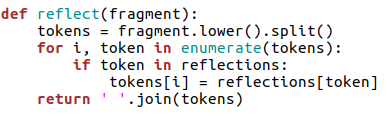
\includegraphics[scale=0.6]{./Pictures/reflect.png}
\caption{Reflect} 
\end{figure}

The first function that appears to us is called reflect. We iterate through the list of tokens and, if the token exists in our dictionary, we replace it with the value from the dictionary.

\item{Analyze}


\begin{figure}[h]
\centering
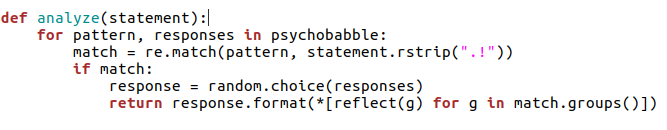
\includegraphics[scale=0.6]{./Pictures/analyze.png}
\caption{Analyze}
\label{fig:analyze}
\end{figure}

The second function that appears is called analyze. We look for if any word in the dictionary match with any word in the user's statement, from which we have stripped the final punctuation. If we find a match, we choose a response template randomly from the list of possible responses associated with the matching pattern. If not, we ask for more information.

\item{Main}

	
\begin{figure}[h]
\centering
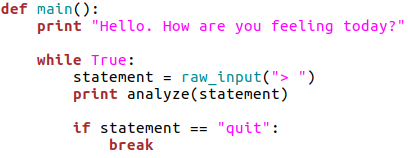
\includegraphics[scale=0.6]{./Pictures/main.png}
\caption{Main}
\label{fig:main}

\end{figure}
Finally, we have the main function that runs the program. First, we show the initial sentence on the screen, to begin the conversation with the user. From there and until the user does not want to stop, we continue having a conversation with him and analyzing his answers with the function presented in figure \ref{fig:analyze}.\\


\item{Example}
	
Here is an example of a the output of the program. We can see exactly what we are referring to in section X. We have given E.L.I.Z.A an entry with the word "child", and it has given us using pattern matching, a response that fits into the conversation. Then we have given E.L.I.Z.A a phrase with words that it does not have in its database and what it has done has been to return a random phrase from the list to continue obtaining information.

\begin{figure}[h]
\centering
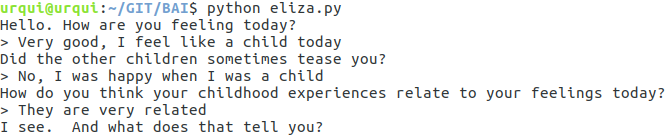
\includegraphics[scale=0.6]{./Pictures/example.png}
\caption{Example}
\end{figure}

We see that the program designed by Mr. Joseph Weizenbaum was a very simple program that response according to previously created templates. With the creation of this program we could already see the first brushstrokes of artficial intelligence in a chatbots.
 
\end{itemize}
		
\subsection{A.L.I.C.E.}
	\label{sec:A.L.I.C.E.}
	is
the Artificial Linguistic Internet Computer Entity, first implemented by Wallace
in 1995. 
	
	If we are talking about chatbots, we can not forget to talk about A.L.I.C.E.. As \cite{shawar2002comparison} says, A.L.I.C.E. (Artificial Linguistic Internet Computer Entity), first implemented by Wallace in 1995,  is a robot that you can make chatting with it. A.L.I.C.E. knowledge is stored in AIML files. AIML is an abbreviation of The Artificial Intelligent Mark up Language that is a derivative of Extensible Mark up Language(XML). Let's see A.L.I.C.E. deeply:


\subsubsection{AIML}

	
	As we can see in \cite{wallace2003elements}, the categories in AIML are the fundamental units of knowledge. A category is at least two more elements, but it can has optional elements. Basic elements are the patterns and templates, which are usually coded in that order (first pattern and second template) because patter would be the question and template would be the answer. The optional context portion of the constant category of variants, called \textless that\textgreater and \textless topic\textgreater. The \textless that\textgreater tag appears within the category, and its pattern must match the last statement of the robot. Remembering a last statement is important if the robot asks a question. The \textless topic\textgreater tag appears outside the category and brings together a group of categories. 
	

	
\subsubsection{Preparation for Pattern Matching}
	\label{sec:preparation}	
	
	Before starting pattern matching procedures each input to the AIML interpreter must pass through two processes:\\
	
	\begin{enumerate}
		\item Normalization Process:
		
		In this step, we intend to retain most of the input information while we adapt that entry to be able to use it well. The recognition of punctuation marks is used mostly and the letters are capitalized. Here we have a table with some examples of this process step by step.
		
		\begin{tabular}{|c|c|c|c|}
			\hline
			 "I like that. :)" & "I like that. " & "I like that" & "I LIKE THAT" \\
			\hline
			\scriptsize{"I don't have. Do you have?"}  & \scriptsize{"I do not have. Do you have?"} & \scriptsize{"I do not have"} & \scriptsize{"I DO NOT HAVE"}\\  &  & \scriptsize{"Do you have?"} & \scriptsize{"DO YOU HAVE"}\\
			\hline
		\end{tabular}
		
		\item Producing input path from each sentence.
		
		This path has the following form:
		
		Input \textless That\textgreater Tvalue\textless Topic\textgreater Pvalue,  where:
		
			\begin{itemize}
			
			\item Input is the normalized input
			\item \textless That\textgreater previous bot answer, normalized in the same way as input
			\item Tvalue is the previous bot answer if exist and * if it doesn't exist.
			\item \textless Topic\textgreater is an optional top level element that contains categories and has a name attribute assign to it, in order to allow interpreter to prefer responses.
dealing with that topic.
			\item Pvalue is the topic name if exists and * if it doesn't exist.
			\end{itemize}
	\end{enumerate}
	
\subsubsection{Pattern Matching Behaviour}
	\label{sec:match}
	
		AIML interpreter try to match word by word in order to get the largest pattern matching, that is, the best one. It uses the Graphmaster. The Grapfmaster consists of a collection of nodes called Nodemappers. These Nodemappers map the branches from each node. The branches are either single words or wildcards. \\ 
		
\textbf{Algorithm : } 
		
		\begin{enumerate} 
		\item Does the Nodemapper contain the key "\_" ?

			\item If so, search the sub graph rooted at the child node linked by "\_".	

		 		\item Try all remaining suffixes of the input following "X" to see if one matches. 
	 			
			\item If no match was found, try:

				\item Does the Nodemapper contain the key "X"? 

					\item If so, search the sub graph rooted at the child node linked by "X", using the tail of the input (the suffix of the input with "X" removed). 
					\item If no match was found, try: 

						\item Does the Nodemapper contain the key "*"? 
						
							\item If so, search the sub graph rooted at the child node linked by "*". 
					\item Try all remaining suffixes of the input following "X" to see if one matches. 
							\item If no match was found, go back up the graph to the parent of this node, and put "X" back on the head of the input. 
							
							\end{enumerate}

						\textit {For completeness there should also be a terminal case: If the input is null (no more words) and the Nodemapper contains the <template> key, then a match was found. Halt the search and return the matching node.If the root Nodemapper contains a key "*" and it points to a leaf node, then the algorithm is guaranteed to find a match.}
						
						
\subsection{Other interestings Chatbots}
	\label{sec:other}
	
	\begin{itemize}
	
	\item In \cite{vinyals2015neural} a sub symbolic chatbot is presented that uses machine learning. It appears that it can handle the general cases of conversation, even questions it didn’t train upon. The strength of the model is that it can be trained end-to-end and thus requires much fewer hand-crafted rules. The authors state that its answers are sometimes on the short side, and that slight variance in semantics can result in inconsistent answers. Another issue we have with such a methodology is that it’s a completely opaque process.
	
	\item  First launched on the internet by Rollo Carpenter in
1997, Cleverbot is a web service that offers the possibility of interacting by chat message with artificial intelligence in real time. It is an intelligent social robot capable of talking about any topic, but its nature does not allow it to carry out processes such as: remembering long conversations or contextualizing; necessary for interaction and conversation.\cite{molinero2013absurdo}
	
	In \cite{molinero2013absurdo} we can read that since 1991, computer programs capable of simulating a human conversation have been awarded with the Loebner prizes. These, are granted those programs that manage to hire an examiner, who is isolated from everything, and who is in front of a computer; which through written text, dialog with him. This test is known as Turing Test \cite{naor1996verification}, and it is the origin of many web services, programs and applications that can be offered to the public, stories such as search assistants, anti spam systems or human understanding interfaces. Of the services of chatbot, or conversational robot of public access existing at present, Cleverbot -www.cleverbot.com- one of the best known and most "human" that exist in the market. And one of the few that has managed to pass the Turing Test with a score higher than 50 \%. This implies that in front of its human counterpart, more than half of examiners mistakenly determined that a person hidden behind a computer was the chatbot, and that the robot was a person.	
	\end{itemize}
 
\section{Types of chatbots}
	\label{sec:types}
	



	\subsection{Sentimental-chatbots}
	\label{sec:sentimental}
	
	Why would we want to add sentiment analysis to our chatbot? The reasons can be several, like adjusting better to the topic of the conversation, getting more natural answers from our chatbot or maybe just develop a chatbot to tell us something to make us feel better, someone to be with in bad times or someone to share happiness with.
	
	But before we start talking about sentimental chatbots, let's talk about sentiment analysis.
	
		\subsubsection{Sentiment analysis}
		\label{sec::sentiment_analysis}
		
		The sentiment analysis is an important factor to take into account in any company, either to adjust our marketing strategy or to improve customer service, for example. Therefore it is also an important factor for any chatbot that works in a company, for example functioning as a chatbot for customer service.\\
		
		Opinion mining is usually called also sentiment analysis. According to Bing Liu from the University of Illinois: \\
		
		\begin{center}
			\textit{"Given a set of evaluative text documents that contain opinions (or sentiments) about an object, opinion mining aims to extract attributes and components of the object that have been commented on in each document d $\in$ D and to determine whether the comments are positive, negative or neutral"} \cite{bingliu_sentiment_definition}.
		\end{center}
		
		In other words, we have some documents containing subjective information and our goal is to evaluate this information in order to assign a sentiment or positiveness value to each comment or document.\\
		
		As B. Pang and L. Lee say, there are several problems in the sentiment analysis \cite{sentiment_analysis_bpang_llee}:
		
		\begin{itemize}
			\item First of all, we have to determine which documents or webpages have relevant information for sentiment analysis, that's opinions, reviews, etc.
			\item Then it comes the problem of which portions of the documents or the information we are analyzing are useful for the sentiment analysis.
			\item After this we have to determine whether the opinion or information expresses a positive or negative feeling, or directly with what feeling it corresponds. In some pages like Amazon it can be easier since in the comments section, each comment is associated with a product evaluation that usually reflects the user's agreement and therefore the degree of positivity of the comment, but in other occasions in which we have no clue can be complicated.
			\item Finally we must internally represent in our chatbot or sentiment analysis program that feeling, since not in all the web pages or documents in which we are given a previous valuation the same measurement system is used (Amazon uses a 5 stars system, Yahoo answers uses a like-dislike system, etc) and we must normalize these values.
		\end{itemize}
	
		There are many tools that allow us or help us to analyze sentiment easily. Most of them are convolutional neural networks trained with huge datasets.
	
		For example, there are already developed free tools that we can use directly in our sentiment analysis like \textbf{"pattern.en".}
		
		\begin{center}
			\textit{"The pattern.en module contains a fast part-of-speech tagger for English (identifies nouns, adjectives, verbs, etc. in a sentence), sentiment analysis, tools for English verb conjugation and noun singularization \& pluralization, and a WordNet interface."} \cite{python_module}
		\end{center}
		
		\begin{figure}[H]
			\centering
			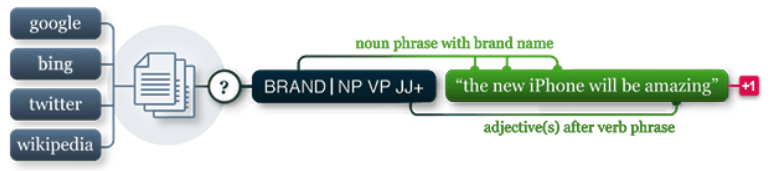
\includegraphics[scale=0.8]{./Pictures/python_module.png}
			\caption{Ilustration of the patter.en python module working.} 
		\end{figure}
	
		Let's take a deeper look into the sentiment section of this module. This module has two functions for sentyment analysis \cite{python_module_sentiment}:
		
		\begin{itemize}
			\item sentiment(sentence): It's the main function for sentiment analysis in this module . As we can read in the webpage \cite{python_module_sentiment}, it gives us two values:
			
			\begin{itemize}
				\item polarity: It takes values from -1.0 to 1.0. It tell us if the sentence is positive or negative. The algorithm is based on the adjectives of the sentence.
				\item subjectivity: It takes values from 0.0 to 1.0.
			\end{itemize}
			
			\item positive(s, threshold=0.1): It returns True if the given sentence's polarity is above the threshold. We can use this function to detect stronger ir lighter sentiments giving different values to the threshold. \textit{"Accuracy is about 75\% for movie reviews" }\cite{python_module_sentiment} so we can see that there are good tools free-to-use in our sentiment analysis. 
		\end{itemize}
		
		In another example, Cicero Nogueira dos Santos and Maira Gatti propose a \textbf{deep convolutional neural network for sentiment analysis of short texts} \cite{glorot2011domain}.\\
		
		In this case the neural network takes a sentence as an input and returns a score for each sentiment label in a set. \\
		
		In order to do that, every word is converted into a vector, which is composed of two sub-vectors:
		
		\begin{enumerate}
			\item Word-level: It captures syntactic and semantic information.
			\item Character-level: It captures morphological and shape information.
s\end{enumerate}
	
		Once we have the sentence converted into word-level and character-level embeddings, the next step they do in CharSCNN consists in extracting a sentence-level representation, but there are two main problems: sentences have different sizes and important information can appear at any position in the sentence. \\
		
		To solve this problem they use a second convolutional layer: \textit{"This layer produces local features around each word in the sentence and then combines them using a max operation to create a fixed-sized feature vector for the sentence."\cite{glorot2011domain}}.\\
		
		Finally, to finish their neural network architecture, this feature vector of the sentence is processed by two neural network layers, which extract one more level of representation and compute a score for each sentiment label. This is the output, as said before.\\
		
		
		
		We can use aswell tools as a help for our algorithms and neural networks in sentiment analysis such as \textbf{"Tweet sentiment application"} \footnote{https://www.csc2.ncsu.edu/faculty/healey/tweet\_viz/tweet\_app/} developed by Dr. Christopher Healey that allows you to search for tweets based on keywords and shows us information about tweets containing those keywords that can be very useful such as Sentiment, Topics, Heatmap, Tag Cloud, Timeline, Map, Affinity, Narrative and tweets. \\
		
		The most useful for us is the Sentiment information that show us a graphic representation of the sentiments shown in the tweets: \textit{"Sentiment. Each tweet is shown as a circle positioned by sentiment, an estimate of the emotion contained in the tweet's text. Unpleasant tweets are drawn as blue circles on the left, and pleasant tweets as green circles on the right. Sedate tweets are drawn as darker circles on the bottom, and active tweets as brighter circles on the top. Hover your mouse over a tweet or click on it to see its text"} \cite{tweet_sentiment_analysis}.
		
		\begin{figure}[H]
			\centering
			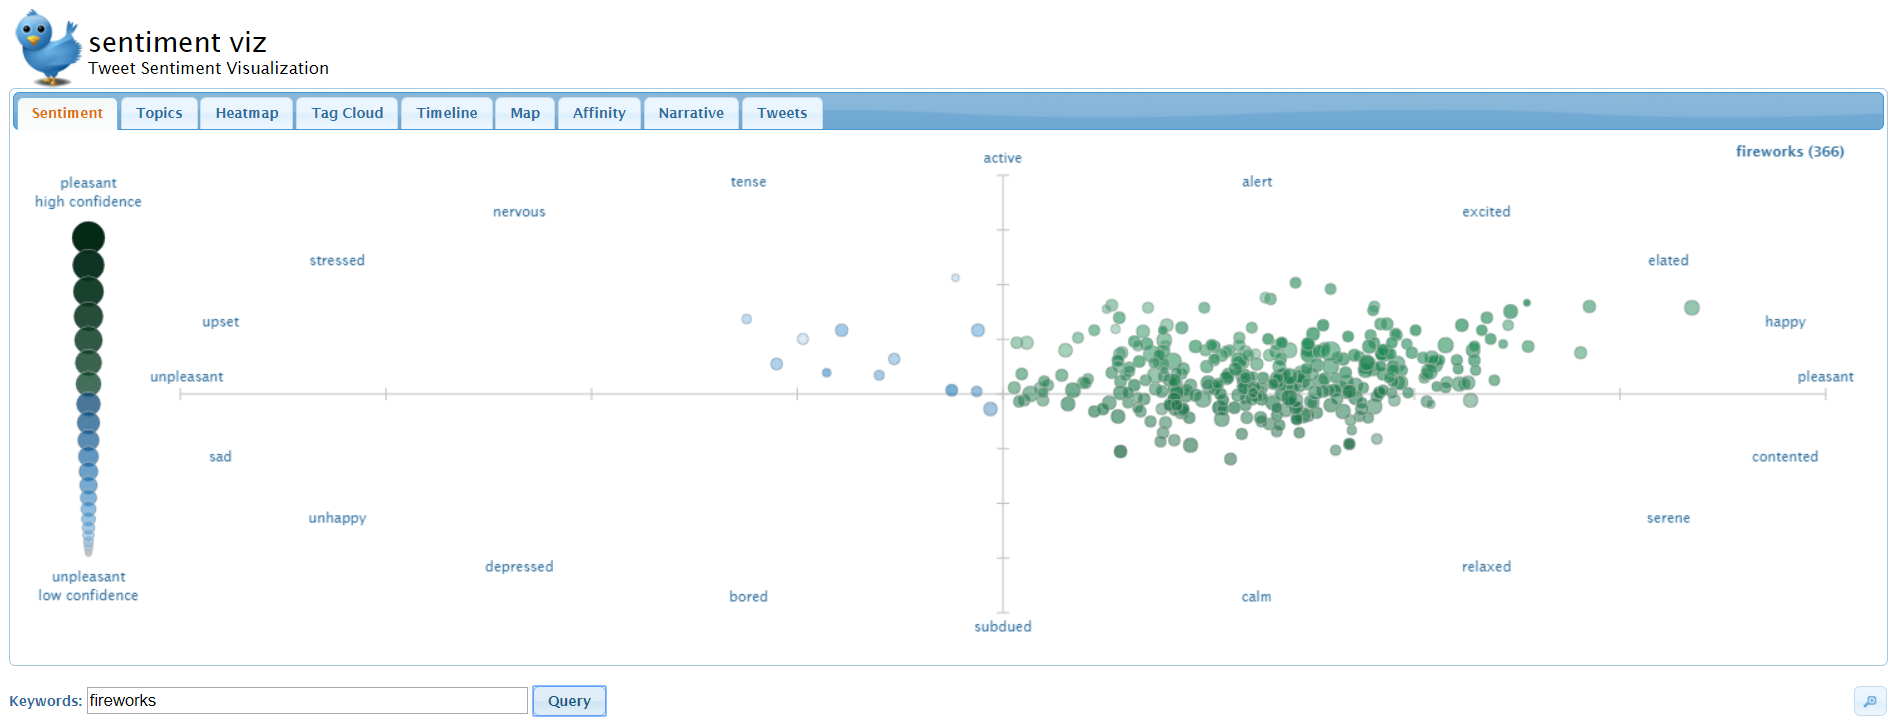
\includegraphics[scale=0.35]{./Pictures/fireworks_sentiment_visualization.png}
			\caption{As we can see, most of the tweets associated to the keyword "fireworks" are positive. This can be usefull when parsing some texts containing some words we don't know how to proccess.} 
		\end{figure}
		
		

	\subsection{Assistant-chatbots}
	\label{sec:assistant}
	
	Now we are going to reseach about Assistant chatbots. As we can read in \cite{imrie2013virtual}, a chatbot with natural language algorithms and localised data could be used as a virtual personal assistant. However, this will require the program to be able to create metadata by forming links between data in given by the user and provide contextual outputs during the interaction that the user finds intersenting and useful. The difference between the way that each chatbot examines the personal data allow us to categorize the apparently similar programs dependind on where the data remains:
	\begin{itemize}
\item \textit{Information service providers: }
They are systems that carry out requets but also provide support for the organisation behind the system. These programs don’t have a localised library for their natural language processing. That means the program is not focusing on each individual user, although the data generated by the analysis of the user activity is saved and controled by the Company. An example of this type og chatbot is Siri from Apple.

\item \textit{Content providers.}
They are systems that provides the information to be used by other systems.  They explore data form existing databases and create its own metadata. They interact with content providers and become into a large data libraries.  

\item \textit{Mediation service:}
They are systems that function as a intermediate between the user and other services. Mediation service could be really useful because it acts as a direct connection between the services and posible multiple users. 

\item \textit{Third party service: }
Contains services that can be applied to a system for its own improvement. This system doesn´t provide services for the users, it gives support for the systems that the user is using.  When this system belong to the user, the third party system can’t interact. Finally, the system could act as an intermediary for the support systems. 

\item \textit{User owned services: }
They work for the user personally, allowing private information keep between the user and the system. The support system does not only have local data and libraries, it also develops metadata and contextual data as a result of use analysis and history of interaction with user. All of contextually developed content in the data library is owned and under the control of the end user.
	
\end{itemize}

\section{Comparison between chatbots and humans}
\label{sec:comparison}

How can we measure if our chatbot is "human" enough? Or how can we see the differences of our chatbot with respect to a human?\\

In 1950, Alan Turing proposed the Imitation Game as a replacement for the question, “Can machines think?” He predicted that by the year 2000 technological progress would produce computing machines with a capacity of log bits, and that with such machinery, a computer program would be able to fool the average questioner for 5 minutes about 70\% of the time \cite{turing2009computing}\\

In chatbots area, we usually measure the "human intelligence" level of chatbots using the turing test.

\begin{figure}[H]
	\centering
	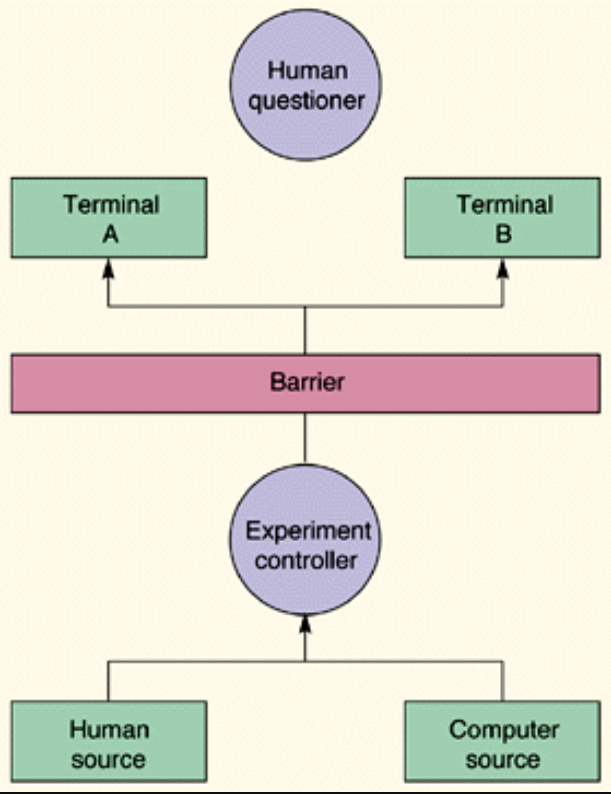
\includegraphics[scale=0.8]{./Pictures/turing_test.png}
	\caption{Graphic ilustration of the turing test.\cite{turing_test_image}}
	\label{fig::turing_test} 
\end{figure}

As we can see, it has the following elements:

\begin{itemize}
	\item An human questioner or tester, who ask questions and chats using 2 terminals.
	\item Two differents sources to chat with: An human source and a computer source that we want to evaluate, int this case a chatbot.
	\item An expermient controller checks if everything is going ok.
	\item A barrier to isolate the tester from the sources.
\end{itemize}

After that, we ask the human questioner which source he thinks it's the human source and which one the computer source. Finally, based on the answers of the testers, we can measure whether the intelligence of our chatbot is enough or not to pass the test.\\

For example, \textit{"Cleverbot passed the 2011 Turing Test at the Techniche TechnoManagement Festival held by the Indian Institute of Technology Guwahati. Of the 1334 volunteers who participated in four-minute typed conversations with either Cleverbot or real humans, 59\% rated Cleverbot as human while 63\% rated the real humans as human (Aron, 2011), suggesting that Cleverbot is one of the most advanced and human-like conversational agents currently available to the public."\cite{HILL2015245}}

\subsection{Loebner prizes}
	\label{sec:loebner}
	
	In \cite{loebner2011} we can read that "The Loebner Prize, named after its founder and philanthropist Hugh Loebner, is an annual world-wide contest to test the state-of-the-art in artificial intelligence (AI)."\\
	


	In 1991, Dr. Hugh Loebner, the National Science Foundation, and the Sloan Foundation started the Loebner Prize Competition: an annual contest between computer programs to identify the most “human’~ programs, and eventually to award \$100,000 to the program that first passes an unrestricted Turing test \cite{epstein1992quest}. This competition has been criticized as a parlor game, rewarding tricks rather than furthering the field of Artificial Intelligence \cite{shieber1994lessons}. \\
	
	For example, those are the last year Loebner prizes:
	
	\begin{itemize}
		\item 2016: Mitsuko created by Steve Worswick
		\item 2015: Rose created by Bruce Wilcox
		\item 2014: Rose 
		\item 2013: Mitsuko
		\item 2012: Chip Vivant! created by Mohan Embar
		\item 2011: Rose
		\item 2010: Alice bot created by Richard Wallace
	\end{itemize}





\section{Conclusion}
\label{sec:conclusion}

We have learned that

%%%%%%%%%%%%%%%%%%%%%%%%%%%%%%%%%%%%%%
% hier werden - zum Ende des Textes - die bibliographischen Referenzen
% eingebunden
%
% Insbesondere stehen die eigentlichen Informationen in der Datei
% ``bib.bib''
%
\nocite{*}

\newpage
\bibliographystyle{alpha}
\addcontentsline{toc}{section}{Bibliography}% Add to the TOC
\bibliography{bib}

\end{document}


